
%%
%% This is file `sample-sigconf.tex',
%% generated with the docstrip utility.
%%
%% The original source files were:
%%
%% samples.dtx  (with options: `sigconf')
%% 
%% IMPORTANT NOTICE:
%% 
%% For the copyright see the source file.
%% 
%% Any modified versions of this file must be renamed
%% with new filenames distinct from sample-sigconf.tex.
%% 
%% For distribution of the original source see the terms
%% for copying and modification in the file samples.dtx.
%% 
%% This generated file may be distributed as long as the
%% original source files, as listed above, are part of the
%% same distribution. (The sources need not necessarily be
%% in the same archive or directory.)
%%
%% The first command in your LaTeX source must be the \documentclass command.

\documentclass[sigconf]{acmart}

\graphicspath{ {./imgs/} }
%%
%% \BibTeX command to typeset BibTeX logo in the docs
\AtBeginDocument{%
  \providecommand\BibTeX{{%
    \normalfont B\kern-0.5em{\scshape i\kern-0.25em b}\kern-0.8em\TeX}}}
    
\usepackage{listings}

\definecolor{mygreen}{rgb}{0,0.6,0}
\definecolor{mygray}{rgb}{0.5,0.5,0.5}
\definecolor{mymauve}{rgb}{0.58,0,0.82}

\lstset{ 
  backgroundcolor=\color{white},   % choose the background color; you must add \usepackage{color} or \usepackage{xcolor}; should come as last argument
  basicstyle=\footnotesize,        % the size of the fonts that are used for the code
  breakatwhitespace=false,         % sets if automatic breaks should only happen at whitespace
  breaklines=true,                 % sets automatic line breaking
  captionpos=b,                    % sets the caption-position to bottom
  commentstyle=\color{mygreen},    % comment style
  escapeinside={\%*}{*)},          % if you want to add LaTeX within your code
  extendedchars=true,              % lets you use non-ASCII characters; for 8-bits encodings only, does not work with UTF-8
  frame=single,	                   % adds a frame around the code
  keepspaces=true,                 % keeps spaces in text, useful for keeping indentation of code (possibly needs columns=flexible)
  keywordstyle=\color{blue},       % keyword style
  morekeywords={*,...},            % if you want to add more keywords to the set
  numbers=left,                    % where to put the line-numbers; possible values are (none, left, right)
  numbersep=-3pt,                   % how far the line-numbers are from the code  
  numberstyle=\tiny\color{mygray}, % the style that is used for the line-numbers
  rulecolor=\color{black},         % if not set, the frame-color may be changed on line-breaks within not-black text (e.g. comments (green here))
  showspaces=false,                % show spaces everywhere adding particular underscores; it overrides 'showstringspaces'
  showstringspaces=false,          % underline spaces within strings only
  showtabs=false,                  % show tabs within strings adding particular underscores
  stringstyle=\color{mymauve},     % string literal style
  tabsize=2,	                   % sets default tabsize to 2 spaces
  title=\lstname                   % show the filename of files included with \lstinputlisting; also try caption instead of title
}

%% Rights management information.  This information is sent to you
%% when you complete the rights form.  These commands have SAMPLE
%% values in them; it is your responsibility as an author to replace
%% the commands and values with those provided to you when you
%% complete the rights form.
%%\setcopyright{acmcopyright}
%%\copyrightyear{2018}
%%\acmYear{2018}
%%\acmDOI{10.1145/1122445.1122456}

%% These commands are for a PROCEEDINGS abstract or paper.
%%\acmConference[Woodstock '18]{Woodstock '18: ACM Symposium on Neural
%%  Gaze Detection}{June 03--05, 2018}{Woodstock, NY}
%%\acmBooktitle{Woodstock '18: ACM Symposium on Neural Gaze Detection,
%%  June 03--05, 2018, Woodstock, NY}
%%\acmPrice{15.00}
%%\acmISBN{978-1-4503-XXXX-X/18/06}


%%
%% Submission ID.
%% Use this when submitting an article to a sponsored event. You'll
%% receive a unique submission ID from the organizers
%% of the event, and this ID should be used as the parameter to this command.
%%\acmSubmissionID{123-A56-BU3}

%%
%% The majority of ACM publications use numbered citations and
%% references.  The command \citestyle{authoryear} switches to the
%% "author year" style.
%%
%% If you are preparing content for an event
%% sponsored by ACM SIGGRAPH, you must use the "author year" style of
%% citations and references.
%% Uncommenting
%% the next command will enable that style.
%%\citestyle{acmauthoryear}

%%
%% end of the preamble, start of the body of the document source.
\begin{document}

%%
%% The "title" command has an optional parameter,
%% allowing the author to define a "short title" to be used in page headers.
\title{Vulnerabilities in WebAssembly: A Survey}

%%
%% The "author" command and its associated commands are used to define
%% the authors and their affiliations.
%% Of note is the shared affiliation of the first two authors, and the
%% "authornote" and "authornotemark" commands
%% used to denote shared contribution to the research.
\author{Holger Klein}
%%\authornote{Both authors contributed equally to this research.}
%%\email{uaidx@student.kit.edu}
%%\orcid{1234-5678-9012}
%%\author{G.K.M. Tobin}
%%\authornotemark[1]
%%\email{webmaster@marysville-ohio.com}
\affiliation{%
  \institution{Karlsruhe Institute of Technology (KIT)}
%%  \streetaddress{P.O. Box 1212}
  \city{Karlsruhe}
%%  \state{Deutschland}
  \country{Germany}
%%  \postcode{43017-6221}
}


%%
%% By default, the full list of authors will be used in the page
%% headers. Often, this list is too long, and will overlap
%% other information printed in the page headers. This command allows
%% the author to define a more concise list
%% of authors' names for this purpose.
\renewcommand{\shortauthors}{Holger Klein}

%%
%% The abstract is a short summary of the work to be presented in the
%% article.
\begin{abstract}
	WebAssembly is a binary bytecode format and compilation target originally designed for use together with Javascript to bring almost native performance to the web. Security mechanisms inherent to the language were a major focus during the design. Structured control flow and managed function return addresses make many popular exploits such as return-oriented programming impossible. However, research has shown that due to the absence of common exploit mitigation techniques, vulnerabilities in high-level languages such as C lead to vulnerabilities in compiled WebAssembly. We introduce the main vulnerabilities and demonstrate proof-of-concept exploits. An overview over the most promising software analysis techniques such as abstract interpretation or fuzzing is presented. We introduce the most up-to-date analysis on real-world WebAssembly binaries. It seems to suggest that many deployed programs have some of the discussed vulnerabilities. Despite this, there are no known widely circulated exploits. We present some reasons as to what might explain this discrepancy.
\end{abstract}

%%
%% The code below is generated by the tool at http://dl.acm.org/ccs.cfm.
%% Please copy and paste the code instead of the example below.
%%

%%
%% Keywords. The author(s) should pick words that accurately describe
%% the work being presented. Separate the keywords with commas.
\keywords{binary exploits, Webassembly, IT Security}

%% A "teaser" image appears between the author and affiliation
%% information and the body of the document, and typically spans the
%% page.
%%\begin{teaserfigure}
  %%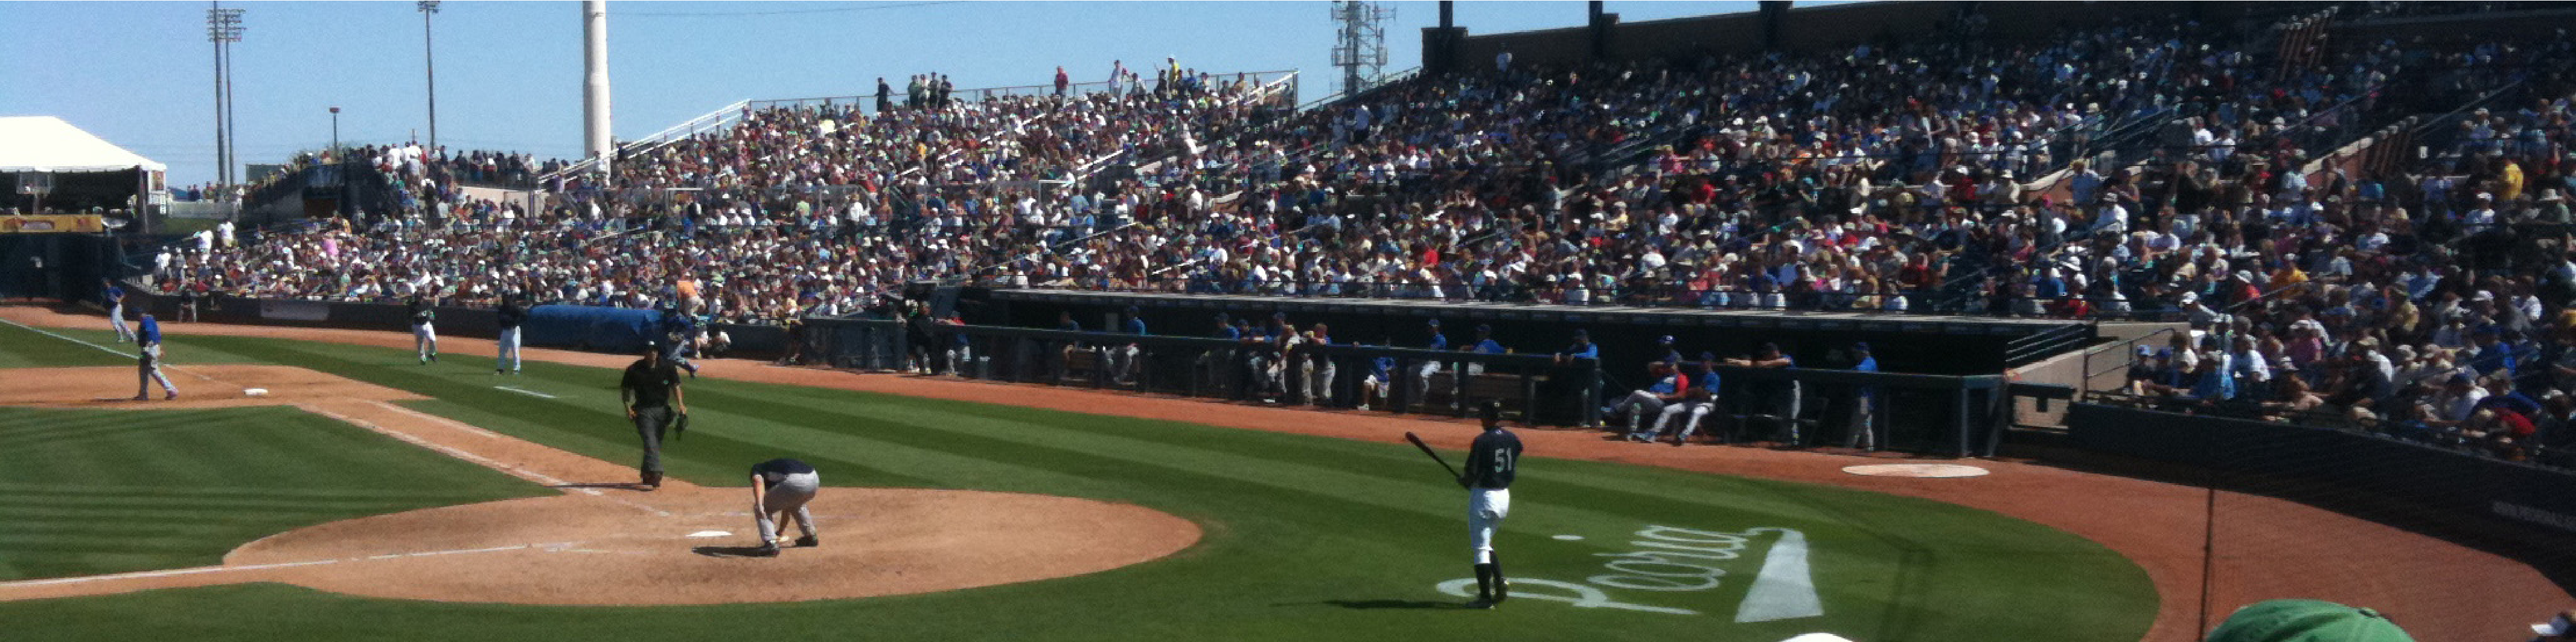
\includegraphics[width=\textwidth]{sampleteaser}
  %%\caption{Seattle Mariners at Spring Training, 2010.}
  %%\Description{Enjoying the baseball game from the third-base
  %%seats. Ichiro Suzuki preparing to bat.}
  %%\label{fig:teaser}
%%\end{teaserfigure}

%%
%% This command processes the author and affiliation and title
%% information and builds the first part of the formatted document.
\maketitle

\section{Introduction}
Introduced in 2018, WebAssembly is a still novel binary code format and compilation target originally meant to bring performance to web applications. The initial design of the API and binary format of WebAssembly got completed in 2017 \url{https://webassembly.org/roadmap/}. Since then, most major browsers such as Firefox, Chrome or Safari implement many of the proposed features. It has since been implemented on other platforms. Even on the server it is possible to run code compiled to WebAssembly when for example using Nodejs. The promise of running code with near native performance in the browser is very attractive, as it allows for more demanding web applications and smoother user experiences. However, since any website visited by the user can download and execute WebAssembly code just like Javascript, it immediately raises security concerns. On the one hand, a malicious website could execute malware on the host computer or use computing ressources by executing a crypto miner. On the other hand, a vulnerable WebAssembly program which takes user input could lead to cross site scripting attacks in the browser. Worse yet, as WebAssebly gets adopted in the backend or even in stand-alone applications, vulnerabilities in WebAssembly programs could enable attacks such as Remote Code Execution. This work will mainly discuss the latter, focusing on how WebAssembly programs might be vulnerable to binary exploitation techniques. In particular, we will focus on how the security mechanisms intrinsic to WebAssembly's design compare to binary exploit mitigations in native applications. As such, this can be seen as a comparison between exploits in native binaries and WebAssembly binaries.

Security is a major selling point of WebAssembly as a platform and was a big concern when it was designed. One publication notes "At worst, a buggy or malicious WebAssembly program can make a mess of the data in its own memory" \cite{rossberg_bringing_2018}. The official spec itself addresses security concerns by stating that "[...] code is validated and executes in a memory-safe*, sandboxed environment preventing data corruption or security breaches". However, it adds a footnote which specifies "*No program can break WebAssembly’s memory model. Of course, it cannot guarantee that an unsafe language compiling to WebAssembly does not corrupt its own memory layout, e.g. inside WebAssembly’s linear memory". Indeed, in the past years there have been puplications commenting on WebAssembly's lack of mitigations for common binary exploitation techniques, such as \cite{mcfadden_security_2018} or \cite{lehmann_everything_2020}. Additionally, there have been puplications researching the real-world assembly programs such as \cite{musch_new_2019} or \cite{hilbig_empirical_2021}. In this work, we aim to cover the main points of these publications and comment on how well WebAssembly is protected against binary exploits by design. We close by presenting the to date biggest analysis on real-world binaries and discuss the apparent lack of widely circulated exploits.

\section{Background}
\label{sec:background}
This survey aims at researching the binary vulnerabilities of WebAssembly. To this end, it is imperative to compare how security mechanisms inherent to WebAssembly compare to security concerns of native binaries. There exists a host of different binary exploitation techniques, and securing against them seems an ever changing arms race between security professionals and hackers. We will mainly concern ourselves with vulnerabilities which are exploited through some malicious form input given by an attacker. These inputs can be a string, file, or key sequence which somehow triggers unexpected behavior in our program. To do so, we will first give an introduction to WebAssembly and how it, as a compilation target, differs from native binary formats and execution environments. Then, we will discuss how this influences typical vulnerabilities such as Stack or Buffer overflows. 

\subsection{WebAssembly}
\label{sec:wasm}
The following will give an Introduction to and and overview of WebAssembly, paying special attention to the parts relevant to a discussion of binary vulnerabilities. For more information, see the official specification at \url{https://webassembly.github.io/spec/core/}, or the Background section in \cite{lehmann_everything_2020}. 

The name 'WebAssembly' (often abbreviated as WASM) is a slight misnomer, since it has a different form and function from typical assembly languages. The official spec refers to it as "low-level, assembly-like". It is a binary byte code format which is interpreted by a Virtual Machine, similar to for example Java. The Virtual Machine is most often implemented in a browser. Design goals were to make WebAssembly safe, hardware- and language independent and fast. In fact, WebAssembly is supposed to run at near-native speeds. There exists a human-readable format of WebAssembly binaries called 'wat'. Whenever we present WebAssembly Code, it will be in this format. While it is possible to hand-craft a wasm binary, it is most often generated by compiling a high-level language such as C/C++ or Rust. In the browser, the binary is then instantiated by calling a Javascript function. See listing \ref{fig:wasm_init_firefox}. By itself, a compiled WebAssembly module has now way of communicating with the host environment such as a Browser (assuming a Bug-free Virtual Machine). Functionality implemented in a WebAssembly module can only be accessed by calling functions which are exported by the module. These exported functions can be called from Javascript code. Conversely, WebAssembly has no I/O other than what is directly supplied through imported Javascript functions. 

\begin{lstlisting}[language=C++, caption={How to intantiate a WebAssembly module using Javascript. (\url{https://developer.mozilla.org/en-US/docs/WebAssembly/Loading_and_running}).}, label=fig:wasm_example_c]
	WebAssembly.instantiateStreaming(fetch('myModule.wasm'), importObject)
	.then(obj => {
		// Call an exported function:
		obj.instance.exports.exported_func();

		// or access the buffer contents of an exported memory:
		var i32 = new Uint32Array(obj.instance.exports.memory.buffer);

		// or access the elements of an exported table:
 		var table = obj.instance.exports.table;
		console.log(table.get(0)());
	})
\end{lstlisting}

\subsection{Modules}
At the highest level, WebAssembly programs are organized into Modules.  A module is the unit which gets compiled and run by the Virtual Machine. Among other things, a module contains definitions for imports and exports, functions, types, tables and memories. All definitions are referenced by zero-based indices. As of the time of writing, only one memory may be defined in a module. This memory is indexed by 0 and implicitly referenced by all other constructs. Memory will be discussed in section \ref{sec:memories}. Also as of time of writing the only table elements which are available are untyped function references. This is used to implement indirect function calls, see section \ref{sec:indirect_calls}. For an example of WebAssembly code, see listing \ref{fig:wasm_example_wasm}.

\begin{lstlisting}[language=C++, caption={A C program, which, when compiled without optimizations, gets translated to the code in Observe \ref{fig:wasm_example_wasm}.}, label=fig:wasm_example_c]
	char *str = "Hello world\n";

	char *indirect_func() {
		return str;
	}

	WASM_EXPORT
	char *direct_func(int i) { 
		char * (*ptr)(void) = &indirect_func;
		return (*ptr)();
	} 
\end{lstlisting}

\begin{lstlisting}[language=C++, caption={The C program in Listing \ref{fig:wasm_example_c} gets compiled to this WebAssembly program (with uninteresting parts removed). Observe the indirect call, function table and memory region.}, label={fig:wasm_example_wasm}]
	(module //start of the module, the unit of compilation in WebAssembly
		(type $t0 (func (result i32)))
		(type $t1 (func))
		(type $t2 (func (param i32) (result i32)))
		(func $__wasm_call_ctors (type $t1))
		(func $indirect_func (type $t0) (result i32) //a function definition
			(local $l0 i32) (local $l1 i32)
			[...]
			i32.load offset=1040
			
			[...]
			return9
		(func $direct_func (export "direct_func") (type $t2) (param $p0 i32) (result i32)
		(local $l0 i32) (local $l1 i32) (local $l2 i32) (local $l3 i32) (local $l4 i32) (local $l5 i32) (local $l6 i32) (local $l7 i32)
		[...]
		call_indirect (type $t0) //calling a function indirectly based on the index pushed onto the stack
		[...]
		return)
	(table $T0 2 2 anyfunc)
	(memory $memory (export "memory") 2) 
	(elem (i32.const 1) $indirect_func) //indirect_func can get called indirectly by pushing '1' onto the stack 
	(data (i32.const 1024) "Hello world\0a\00") //A string in memory. There exists no constant storage in WebAssembly.
	(data (i32.const 1040) "\00\04\00\00"))
\end{lstlisting}

\subsection{The Stack}
\label{sec:wasm_stack}
The WebAssembly virtual machine is conceptually stack based. In contrast to most native platforms, it doesn't have a notion of registers. Instead, values are pushed on and popped off the stack. Many instructions implicitly operate on the stack. See listing \ref{fig:wasm_example_wasm} for an example.

\subsection{Control Flow}
\label{sec:wasm_control_flow}
In contrast to native languages or even Java, WebAssembly enforces so-called 'structured' control flow. Code can only be organized into blocks. Control-flow commands such as those generated by loops can only jump to the beginning of such a block, and only within the current function. In addition, the bytecode has no way of interacting with the underlying addresses of functions. These are only accessible to the Virtual Machine. This immediately makes many binary exploits impossible, such as Return-Oriented Programming. 

\subsection{Memories} 
\label{sec:memories}
WebAssembly only supports four different primitive types: 32- and 64-bit Integers (i32, i64) and single- and double-precision floating point nubmers (f32, f64). As such, arrays, pointers, etc. have no explicit representation at the binary level. To see how they are implemented in binary programs, it is necessary to understand the way WebAssembly handles memory. The implementation of function pointers or virtual functions is discussed in section \ref{sec:indirect_calls}. The stack space of a function which contains the return address as well as any native data types whose address is never taken cannot be accessed to the program. As mentioned in section \ref{sec:wasm_control_flow}, this in itself contributes to WebAssemblys inherent security. However, anything other than a scalar value or any value whose address is taken needs to reside in the so-called linear memory. This memory is a linear array of raw bytes. Addresses are referenced by 32 bit integers which serve as the pointer type. The WebAssembly program can request more memory from the Host VM using the memory.grow operation. The linear memory is completely unmanaged. The way it is used is completely up to the program. Many WebAssembly toolchains such as emscripten (\url{https://emscripten.org/}) include an allocator which implements functions such as C's malloc and free. This unmanaged, linear memory is the main reason for most vulnerabilities discussed in \cite{lehmann_everything_2020}. This will be elaborated in section \ref{sec:binary_vulns}.

\subsection{Indirect Function Calls} 
\label{sec:indirect_calls}
To implement indirect function calls, any function which may get called indirectly or used as a function pointer has an entry in the module's table section. The call\_indirect operation pops an index from the stack which is used to reference an entry in the function table section. This table maps the index to a function. This limits which functions can be called indirectly, as the only functions available are the ones in this table. Listing \ref{fig:wasm_function_addr} shows example code to make this more intuitive. The code prints 1,2,1,3 to the console when running it in the browser.

\begin{lstlisting}[language=C++, caption={This Code demonstrates how WebAssembly handles function pointers. This code prints 1,2,1,3 to the console when running it in the browser.}, label={fig:wasm_function_addr}]
	#include <stdio.h>
	#include <emscripten.h>

	void printLine(const char *s) {
		printf("%s\n", s);
	}

	void printInteger(const int i) {
		printf("%i\n", i);
	}

	int main() {
		printf("%i\n", &printLine);
		printf("%i\n", &printInteger);
		printf("%i\n", &printLine);
		printf("%i\n", &emscripten_run_script);
		return 0;
	}
\end{lstlisting}

Additionally, functions in WebAssembly are type checked. The call\_indirect operation has the function type statically encoded. Thus, this operation can only call functions which have the matching signature. It must be remarked however that this is less limiting than it might first appear, since WebAssembly only has four native types. Thus, a function taking a pointer (or a string) has the same signature as a function taking an 32-bit Integer. This is demonstrated by the code in listing \ref{wasm_function_type_checking}. By copying the index of different functions directly into the function pointer, different functions get called indirectly. The function pointer supposedly takes a pointer to a char as argument. However, it is possible to use the index of a function taking an Integer as parameter. 

\begin{lstlisting}[language=C++, caption={Example demonstrating how function pointer type checking works.}, label={fig:wasm_function_type_checking}]
	#include <stdio.h>
	#include <emscripten.h>
	#include <cstring>

	struct FunctionStruct {
		void (*f) (const char *);
	};

	void printLine(const char *s) {
		printf("%s\n", s);
	}

	void printInteger(const int i) {
		printf("%i\n", i);
	}

	int main() {	
		//using the adresses so they get put in the function table
		printf("%i", &printLine);
		printf("%i", &printInteger);
		printf("%i\n", &emscripten_run_script);
		
		FunctionStruct fs;
		char *printLineIndex = "\x01\x00\x00\x00";
		memcpy(&fs, printLineIndex, 4);
		//prints "printing line" to the console
		fs.f("printing line"); 
		
		char *printIntegerIndex = "\x02\x00\x00\x00";
		memcpy(&fs, printIntegerIndex, 4);
		//prints 1059 to the console
		fs.f("");
		
		char *runscriptIndex = "\x03\x00\x00\x00";
		memcpy(&fs, runscriptIndex, 4);
		//displays an alert
		fs.f("alert('alert')");		
		
		return 0;
	}
\end{lstlisting}

\subsection{Deployment, Compilers and Toolchains}
It would be very impractical (albeit possible) to write WebAssembly from scratch. Thus, several Backends exist to generate WebAssembly bytecode from high-level languages such as C, Go or Rust. Emscripten can not only generate WebAssembly bytecode from C/C++ but also generate Html and Javascript to load and run the WebAssembly module. It also comes with C Headers to interact with the Browser and implements several common libraries such as SDL1 \url{https://www.libsdl.org/} and a wrapper to simulate Linux sockets using webSockets.  

\section{Vulnerabilities of WebAssembly programs}
\label{sec:binary_vulns}
In this section we will discuss the security vulnerabilities of WebAssembly as presented in \cite{mcfadden_security_2018} and \cite{lehmann_everything_2020}. \cite{lehmann_everything_2020} begin by discussing the security-critical aspects of the linear unmanaged memory. As mentioned in section \ref{sec:memories}, every scalar value whose address is never taken, as well as function return addresses are completely managed by the virtual machine. This mitigates many well-known attacks. However, all non-scalar types such as arrays or any value whose address is ever taken must lie in the unmanaged memory. This memory is usually controlled by an allocator provided by the compilation toolchain. Most allocators separate the memory in three distinct regions: The stack, heap and data sections, similar to binary formats such as ELF. To distinguish between the function call stack managed by the VM and the call stack created by the compiler, \cite{lehmann_everything_2020} call the latter the \textbf{unmanaged} stack. We will use the same nomenclature here. One must keep in mind however, that there are no underlying mechanisms provided by the VM to separate between these three regions. This separation is only implemented by the compiler. From the point of view of the platform, it is just a single contiguous linear array of bytes. 

\subsection{Exploit mitigations in native and Webassembly binaries}
\cite{mcfadden_security_2018} discuss serveral common exploit mitigation techniques which are used in binary programs. Table \ref{table:exploit_mitigation_wasm} provides a summary and shows whether these techniques or some replacement are present in WebAssembly. 

\begin{table*}
\begin{tabular}{p{2cm} | p{2cm} | p{6cm} | p{6cm} }
  \toprule
  Exploit mitigation & Protect against & Effect in Native Binaries & WebAssembly \\
  \midrule
  Address Space Layout Randomization (ASLR) & Attacks on Control-Flow & Randomizes the base address of an executable as well as the heap and stack addresses and addresses of libraries. This is meant to make exploitation techniques such as return oriented programming harder. It also makes exploiting other vulnerabilities more challenging& ASLR has no equivalent mechanism in WebAssembly. However, since the user can't access return addresses, many exploits that rely on changing control flow are impossible. In addition, since WebAssembly only provides 32-bit addresses, it is assumed to have too little entropy for ASLR to be effective. Also, since functions are directly accessed by indices instead of memory addresses, ASLR could not be used to obfuscate function addresses. \\ \hline
   Stack Canaries & Stack-based Buffer overflows & Stack Canaries are placed on the stack such that a stack-based buffer overflow will overwrite them before corrupting the functions return address. This enables the program to detect and handle these overflows & Stack canaries don't exist in WebAssembly, since the return addresses are entirely managed by the VM \\ \hline
   Heap Hardening & Manipulating Allocator Metadata & Heap Hardening comprises several different programming techniques to make Allocators more secure against attacks. By corrupting heap metadata, an attacker can use the allocator to execute arbitrary writes on the heap. & Since size is a concern, many toolchains come with the options to compile with their own, smaller allocator which might have vulnerabilities.\\ \hline
   Data Execution Prevention (DEP) & Code injection & This mitigation is part of a family of mitigation techniques which modify memory pages to only allow certain behavior. These can, for example, modify whether the contents of certain memory pages can be executed. In native binaries, this can prevent the injection of malicious code & In WebAssembly, there is a strict separation between code and data. Hence, DEP is not needed (or in other words, always implemented).
\end{tabular}
\label{table:exploit_mitigation_wasm}
\caption{A summary of exploit mitigation techniques commonly found in native binaries. They are compared to their WebAssembly counterparts, if any exist.}
\end{table*}

\cite{lehmann_everything_2020} also discuss common mitigations such as ASLR and page protection flags which are not present in WebAssembly. In particular, since there are no guard pages between the different sections of the linear memory , an overflow in any section can corrupt data in any other section. And since there is no concept of read-only memory, even data which is marked as constant in the source code can be overwritten during execution. In summary, the unmanaged, linear memory has the biggest potential to lead to exploits.

\section{Exploiting Vulnerabilities}
Having analyzed WebAssemblys main vulnerability, the unmanaged linear memory, there are several ways to exploit it. \cite{mcfadden_security_2018} show two attack primitives, format-string attacks and stack-based buffer overflows. They use these attack primitives to implement a proof of concept of a cross-site scripting attack, and remote code execution on a server.
\cite{lehmann_everything_2020} similarly first demonstrate two write primitves. They introduce a stack-based buffer overflow. They also demonstrate how the allocator supplied by emscripten (called emmalloc) is susceptible to the so-called 'unlink exploit'. Given the right circumstances, this can be utilized to allow an attacker to write an arbitrary value to an arbitrary address. However, their exploit didn't work on our machine using version 1.39.16.of emscripten. They also describe how user-supplied data could lead to a stack overflow. Since WebAssembly has no guard pages, a stack overflow could overwrite data following the stack. However, no example of an exploit is given. 

We will quickly summarize the presented attack primitives. Since the one of the main sources of security of WebAssembly comes from the fact that it is isolated from the surrounding environment by the Virtual Machine. Thus, for an exploit to be dangerous in the browser it needs to manipulate data that gets passed to functions which can have an effect outside the isolated program. In the browser, such functions will be imported from Javscript. Examples are functions such as eval or functions which manipulate the DOM.
Eval is a Javascript function which will execute any string passed to it as Javascript code. 

\subsection{Overflowing the unmanaged stack}
\label{sec:stack_buffer_overflow}
Overflowing buffers on the stack is one of the most widely used binary exploitation techniques. It can happen whenever user-supplied data is copied into a buffer on the stack (such as a fixed-size array) without checking the bounds. The most common example of a function which has this vulnerability is the C function gets. The Linux manual even states "never use gets". There are many ways to exploit a stack based buffer overflow. In native binaries without exploit mitigation techniques such as stack canaries, a buffer overflow can be used to overwrite the functions return address. This can allow an attacker to execute arbitrary code with the permissions of the program. However, since the WebAssembly VM manages return addresses separately, one could assume that stack based buffer overflows aren't security concerns for WebAssembly programs. However, if the function has non-scalar data, this will reside in unmanaged memory. In fact, since there exist no stack canaries in WebAssembly, a buffer overflow can overwrite any unmanaged memory above the function's stack frame. This can even include parent frames. Additionally, there are no guard pages in WebAssembly so a stack based buffer overflow can grow into other memory regions such as the heap. And, since there is no concept of read-only data in WebAssembly, any data on the unmanaged stack can potentially be overwritten. \cite{lehmann_everything_2020} have several examples to demonstrate this vulnerability. Listing \ref{fig:vuln_example_stack_overflow} shows an example inspired by their work. The main function generated a string which gets added to the DOM. Before then, it calls a vulnerable function. The user provided input can overflow the stack of the vulnerable function and into the stack of the main function. There, it can overwrite the string added to the DOM. This can lead to a cross site scripting attack.

\begin{lstlisting}[language=C++, caption={This c program has a stack overflow vulnerability. This can be exploited by the user supplying a buffer which overflows into the parent frame and replaces the string meant to be added to the DOM.}, label={fig:vuln_example_stack_overflow}]
	#include <emscripten.h>
	#include <stdio.h>
	#include <string.h>

	void vulnerable() {
		char buffer[8];
		//imagine getting this from the user
		char *data = "aaaaaaaaaaaaaaaaaaaaaaaaaaaaaaaa<script>alert('hello')</script>";
		strcpy(buffer, data);
	}

	void generateHTML(char *buffer) {
		char *welcomeMsg = "<p>welcome to my website</p>";
		strcpy(buffer, welcomeMsg);
	}

	int main() {
		char html[512];
		generateHTML(html);
		vulnerable();
		add_to_dom(html);
		return 0;
	}
\end{lstlisting}

\subsection{Redirecting Control Flow}
Can we influence the program control flow using an overflow as introduced in section \ref{sec:stack_buffer_overflow}? Since the return addresses are managed by the VM, the answer seems to be no. However, it is possible to overwrite indirect function calls. As discussed in section \ref{sec:indirect_calls}, WebAssembly references functions by an Integer. The indirect function call can be influenced if two conditions are met:

\begin{itemize}
\item The Integer which identifies the called function lies somewhere in unmanaged memory.
\item The originally called function has the same arguments and return type as the newly called function.
\end{itemize}

Also, if we wish to influence the parameters passed to the newly passed function they too must be within unmanaged memory. The most interesting fact is that, since WebAssembly has no way to mark memory as read-only, it is possible to overwrite supposedly constant data. \cite{mcfadden_security_2018} demonstrate a proof of concept of using a overflow to manipulate control flow. We couldn't recreate their exact example, however a slight modification did work. The example in listing \ref{fig:vuln_example_redirect_control_flow} works on Firefox version 88.0.1 64-Bit when compiled with emscripten version 1.39.16.

The proposed scenario is that of a legacy application being ported to WebAssembly. It is possible to send messages and handle them using different functions. A especially crafted payload can be used to overflow into the {msg\_len and out fields, changing the program behavior. It exploits an unchecked memory copy to alter the control flow. This is used to implement a cross-site scripting attack. When the code is executed in the browser, it displays an alert. Of course, one can imagine reworking this exploit to steal cookies, etc.
The example is particularly interesting since it could only work in WebAssembly and not on other native platforms.

\begin{lstlisting}[language=C++, label=fig:vuln_example_redirect_control_flow, caption={This code demonstrates a proof of concept of an exploit using indirect calls to influence control flow and implement cross site scripting. Taken with modifications from \cite{mcfadden_security_2018}}]
	#include <stdio.h>
	#include <emscripten.h>
	#include <stdint.h>
	#include <cstring>

	struct Communication {
		char msg[64];
		uint16_t msg_len;
		void (*out) (const char *);
	};

	void printCommunication(Communication * comms) {
		comms->out(comms->msg);
	}

	void printLine(const char *msg) {
		printf("%s\n", msg);
	}

	int main() {
		//use adress hereso it gets added to the import table
		printf("%i\n", &emscripten_run_script); 

		Communication comms;
		comms.out = &printLine;
		
		char *payload = "alert('XSS');// " 	//16 byte attack script
						"                " 	//16 byte padding
						"                " 	//16 byte padding
						"                " 	//16 byte padding
						"  "				//2 byte padding
						"\x40\x00"         	//msg_len=68
						"\x01\x00\x00\x00";	//out=1
						
		memcpy(comms.msg, payload, 72);
		printCommunication(&comms); //trigger the exploit
		
		return 0;
	}
\end{lstlisting}

\section{Binary Analysis}
\subsection{Native Binaries}
Trying to decide whether a given program will crash is equivalent to the Halting problem. Thus, automating the discovery of binary vulnerabilities is a hard problem. We will first give some background on different techniques that have been developed for native binaries. Then, we will show which solutions exist for WebAssembly. A thorough summary of these techniques is outside the scope of this work, however we aim to give an intuitive understanding for the techniques used in the state of the art. See for example \cite{sun_new_2018} for a more thorough review.

Techniques to discover binary vulnerabilities can roughly be divided into two categories: Static and dynamic analysis techniques \cite{shoshitaishvili_sok_2016}. A concept which will be interesting in this discussion is representing programs as Control Flow Graphs (CFGs). In such a graph, the nodes are instructions and the edges possible execution flows between these instructions. There exist algorithms to automatically generate CFGs from binary programs. This is, however, not an exact science. One problem is deciding how to trade-off false positive edges. This is especially the case when dealing with indirect or conditional jumps. While a CFG with zero edges would have no false positives, a CFG with edges between any two program instructions would surely contain all possible jumps as well as many false positives. Clearly, the ideal is somewhere in between these two extremes.

\begin{lstlisting}[language=C++, label=code:control_flow_example, caption={This pseudocode corresponds to the control flow graph in Figure \ref{fig:vuln_example_redirect_control_flow}}]
	void f() {
		while(n < 1000) {
			n := n + 1;	
		}
	}
\end{lstlisting}

\begin{figure}[h]
  \centering
  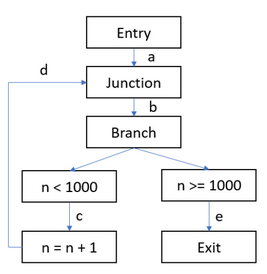
\includegraphics[height=5cm]{control-flow-graph}
  \caption{A Control Flow Graph derived from the Pseudocode in listing \ref{code:control_flow_example}}  
\label{fig:vuln_example_redirect_control_flow}
\end{figure}

Static program analysis techniques reason about the program without executing it. Thus, the analysis has to reason about the properties of the program by abstracting it. The biggest analysis trying to find vulnerabilities in real-world WebAssembly programs undertaken thus far utilizes static analysis with a heuristic. It will be discussed in section \ref{sec:real_world_wasm_analysis}.

Dynamic binary analysis techniques on the other hand work by executing the program for some input and observing its behavior. Generating these inputs is most commonly done by a tool called a Fuzzer \cite{li_fuzzing_2018}. Fuzzers aim to generate inputs that trigger interesting behavior in the target program. Creating a Fuzzer which generates input that successfully triggers crashes is far from trivial. At a high level, Fuzzers are either coverage or taint based. Coverage based Fuzzers aim at generating inputs which maximize the percentage of executed code. Taint based Fuzzers analyze which parts of the code are influenced (tainted) by user input. These analyses require some understanding of the source program. Thus, it seems natural that effective Fuzzers utilize some kind of static analysis. Thus, the separation into static and dynamic techniques isn't very strict.

An analysis method which lies somewhere in between static in dynamic methods is is abstract interpretation. Abstract interpretation is a based on programming language semantics and their fixed points \cite{cousot_abstract_2000}. Intuitively, the program is run in a way where using all possible values of a given type. For example, instead of running a program using integers as a type, intervals are used. The  operands defined on the original type are also adjusted to act on the abstract value type. 

A popluar open-source framework to implement binary analysis techniques is the python-based angr, introduced in \cite{shoshitaishvili_sok_2016}. It provides tools for loading binaries, computing CFGs, etc. \cite{boudjema_vyper_2020} builds on angr to implement VYPER, a tool which utilizes concolic execution of the binary target. This is done to lower the amount of false positives. 

There has also been work trying to utilize deep neural nets to locate faults in native binaries, for example \cite{li_locating_2019}.

\subsection{WebAssembly Binaries}
\label{sec:wasm_analysis}
There are several tools and approaches to specifically analyze WebAssembly Binaries to locate vulnerabilities. One proposed tool, Wasmati, is introduced in \cite{lopes_discovering_2021}. It aims to utilize Code Property Graphs. While promising, it has yet to be implemented and tested. TaintAssembly, introduced in \cite{fu_taintassembly_2018} tracks taint through binaries using a modified V8 Javascript Engine. This comes with some limitations however such as not propagating indirect taint. It also seems like it wasn't ever evaluated on finding vulnerabilities in real-world vulnerabilities. \cite{sun_poster_2021} describes a deep neural net architecture to find vulnerabilities in WebAssembly binaries, the WASP framework. However, it has yet to be evaluated on more real-world binaries. Preliminary results seem promising, however. 

Wasabi \cite{lehmann_wasabi_2018} is a Rust-based tool aimed at enabling the writing analyses of WebAssembly binaries. The analysis code is written in Javascript by utilizing hooks provided by the framework. The WebAssembly instructions are grouped to make writing analyses easier. Thus, for example, there is one hook for all function calls. If present, a user-implemented callback function is triggered on WebAssembly function calls while the function name and other information gets passed to the callback. Only those hooks which are implemented in the Javscript analysis get put into the binary to improve performance. Wasabi is the basis for the static analysis tools presented in \cite{lehmann_everything_2020} and also used in \cite{hilbig_empirical_2021}. This tool performs static analysis utilizing heuristics to try and find possible vulnerabilities. Using the Rust-based Wasabi implementation as a library, the stack pointer in a given binary is identified. This is done using a heuristic which looks for a variable of type i32 which is mutable, written to and read from globally, and has at least three reads and writes to avoid false positives in small binaries. This heuristic seems to work well when checked against to manual verification. To identify possible vulnerabilities the tool looks for either of the following: use of unmanaged memory as introduced in section \ref{sec:wasm_stack}, unsafe memory allocators such as emmalloc (see section \ref{sec:binary_vulns}) or importing potentially dangerous functions such as eval.

\section{Analysis Real-World WebAssembly Binaries}
\label{sec:real_world_wasm_analysis}
To date, there exist three major analyses of different aspects of WebAssembly binaries "in the wild": One from 2019 \cite{musch_new_2019}, focused on the way WebAssembly is used by the 1 million most visited websites. \cite{lehmann_everything_2020} uses the WebAssembly static analysis tool explained in \ref{sec:wasm_analysis} on real-world WebAssembly programs to ascertain whether the vulnerabilities they discuss exist in deployed code. Finally, in 2021 \cite{hilbig_empirical_2021} ran the thus far largest analysis combining the methods of both \cite{musch_new_2019} and \cite{lehmann_everything_2020}. Since their results refine the previous work and comprise a much larger dataset (8,461 unique WebAssembly binaries), we will focus mainly on their work. Afterwards, we will discuss their findings in section \ref{sec:discussion}. 

Regarding the use of the unsafe, unmanaged memory, 65\% of the analyzed programs make use of it, see figure \ref{fig:analysis_unmanaged_stack}. Looking at the use of potentially unsafe memory allocators, only 11 binaries use emmalloc. 38,6\% of all binaries use custom, unknown allocators. Of the known, non-standard allocators, 37\% are from EOSIA, a WebAssembly platform for smart contracts. See figure \ref{fig:analysis_used_alloc}. Figuring out whether these allocators have exploitable vulnerabilities requires further research. The final heuristic concerns imported functions which are potentially harmful. They separate these functions into categories such as file I/O or code execution. While 21,2\% of the binaries import at least one potentially harmful function, the overwhelming majority of these cases (in 19\% of all binaries) are I/O functions. 

\begin{figure}[h]
  \centering
  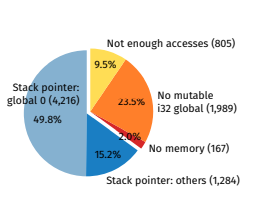
\includegraphics[scale=1]{analysis_unmanaged_stack}
  \caption{Result of an analysis of memory usage in real world WebAssembly binaries, taken from \cite{hilbig_empirical_2021}.}  
\label{fig:analysis_unmanaged_stack}
\end{figure}

\begin{figure}[h]
  \centering
  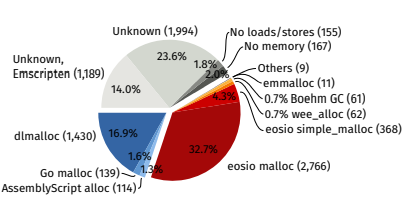
\includegraphics[scale=1]{analysis_used_alloc}
  \caption{Result of an analysis of allocators used in real world WebAssembly binaries, taken from \cite{hilbig_empirical_2021}.}  
\label{fig:analysis_used_alloc}
\end{figure}

\begin{table*}
\label{table:analysis_import_harmful_functions}
\caption{Result of an analysis of potentially harmful functions imported into WebAssembly modules. Taken from \cite{hilbig_empirical_2021} with some modifications.}
\begin{tabular}{l|l|l}
  \toprule
  Category & Patterns & Matches\\
  \midrule
  Code execution & eval, exec, execve, emscripten\_run\_script & 1.9\% \\ \hline
  Network access & xhr, request, http, fetch & 2.0\% \\ \hline
  File I/O  & file, fd, path & 19.0\% \\ \hline
  Dynamic linking & dlopen, dlsym, dlclose  & 1.6\%
\end{tabular}
\end{table*}

\subsection{Discussion}
\label{sec:discussion}
Given the results of the analysis presented in section \ref{sec:real_world_wasm_analysis}, it seems quite a lot of real-world WebAssembly binaries are potentially vulnerable. Despite this, it seems there are no known, widely deployed exploits targeting WebAssembly binaries. Using exploitdb (\url{https://www.exploit-db.com/}) and searching for either the terms 'wasm' or 'webassembly' yields one and three results, respectively. The latter date back to 2018, the former to 2019. Additionally, all of them are exploits targeting the VM, not a WebAssembly Binary using some malicious input. Similarly, using google to search for the terms 'exploit webassembly', or 'webassembly binary exploit' doesn't yield any exploits on the first three pages. Given that \cite{mcfadden_security_2018} discussed potential WebAssembly vulnerabilities as far back as 2018, the question remains as to why there haven't been more exploits widely reported on. Especially regarding the fact that binary security remains one of the major selling points of WebAssembly, one would expect the discovery of an effective exploit in the wild to be widely shared and discussed. This seems to suggest that the unavailability of information regarding exploits correlates to there not being any. In what follows, we suggest reasons for why that might be with suggestions regarding how to test these hypothesis where applicable.

\subsubsection{The analyses are incomplete}
\label{sec:analyses_incomplete}
One reason that might explain the discrepancy between the many binaries which have at least one apparent vulnerability and the lack of exploits in the wild is that the analyses we discussed are leaving out some important factor which makes exploits way less likely. For example, many of the binaries which import some dangerous function might never take any user input which might exploit them. The way to test this would be to test the collected binaries as to whether they take user input and which parts of the code are affected by this input. This could use the taint analysis discussed in \ref{sec:wasm_analysis}. It would be interesting to see how many binaries use both unmanaged memory, import an unsafe function, and allow user supplied input to affect the programs behavior. This could be an interesting avenue for future work. The analysis done so far rely on static analysis and a heuristic, which isn't sophisticated compared to state-of-the-art program analysis techniques available for native binaries.

\subsubsection{There are easier or more lucrative targets}
\label{sec:better_targets}
Since many WebAssembly modules are only available as binaries, interpreting them well enough to find exploits might have significant overhead compared to exploiting Javascript. Additionally, it stands to reason that the vast majority of Websites still mainly rely on Javascript to handle their business logic in the front and backend. And finally, the way WebAssembly is often discussed seems to suggest using it to only speed up the critical code paths and calling into the WebAssembly code from Javascript. Although this is less true when using Emscripten, which for example has functionality to write main functions or define update-render loops for games. All this seems to point towards the fact that people interested in potentially exploiting WebAssembly would find it easier and more profitable to instead focus on Javascript or native binaries. Again, this is conjecture, and hard to either verify or debunk. One could perhaps interview industry experts.

\subsubsection{WebAssembly's security measures are enough}
\label{sec:wasm_sec_strong}
It might also be the case that the structured control flow, managed addresses, together with the sandboxed memory already lead to sufficient security. While the vulnerabilities discussed in \ref{sec:binary_vulns} are valid and enable proof of concept attacks, they might still be impractical. For example, changing control flow requires that: (i) the function's address is on the unmanaged stack, (ii), some data given by the user can override that location, and (iii), another function exists with the same signature which the user can exploit. This reasoning is similar to the points given in sections \ref{sec:analyses_incomplete} and \ref{sec:better_targets}. Thus, having the VM handle return addresses might be enough to hinder most control flow attacks. In addition, a very specific set of circumstances has to occur for a WebAssembly vulnerability to be exploitable, for example by enabling a cross site scripting attack. For example, another user (the victim) would have to trigger an exploit by calling WebAssembly with malicious input somehow supplied by the attacker. It needs be remarked that \cite{lehmann_everything_2020} indeed show an example of cross site scripting being enabled by exploiting a well-known bug CVE-2018-14550 in an image conversion library libpng. When using version 1.6.35 of this library and converting an PNM to a PNG file, there exists a buffer overflow vulnerability. If a website were to use this library to allow users to convert images, and an attacker were to supply malicious input, this overflow could be used to overwrite a string which gets later added to the DOM. Additionally, they compare the control flow defense inherent in WebAssembly to defenses deployed by native binaries, so called control-flow integrity (CFI) policies. They conclude that "Overall, WebAssembly’s type checking is often less effective than modern CFI defenses available for native binaries". However, as mentioned before, diverting control flow in WebAssembly presupposes the ability to taint a very specific part of program memory. Again, testing this hypothesis doesn't seem straightforward. It would probably need both more analysis both automated and manually by experts in the field.

Given more time, it seems likely that whether WebAssembly allows for more exploits than expected will come to light as more and more Websites start using it. Wider adoption would make finding exploits more lucrative and thus, more likely. It seems plausible that the reason why there haven't been any widely talked about WebAssembly exploits (especially following the publication of \cite{lehmann_everything_2020}) is due to a mixture of the factors discussed above.

\section{Conclusion}
We introduced WebAssembly binary format and execution environment, especially regarding possible vulnerabilities. The security measures inherent to WebAssembly such as structured control flow and managed addresses are a selling point of WebAssembly. Despite that, using unmanaged memory in combination with indirect calls and the lack of common exploit mitigation techniques, we demonstrated the existence of proof of concept attacks. These would, for example, enable cross site scripting in certain cases. Discussing a large analysis on real world WebAssembly programs which comprises over 8000 binaries, we showed that a large percentage of them have some of the vulnerabilities introduced before. This leads to an apparent contradiction when considering the fact that there haven't been any widely reported exploits unique to WebAssembly. We concluded by presenting possible reasons as to why that might be and some avenues for future research. 

\bibliographystyle{ACM-Reference-Format}
\bibliography{Wasm-Vuln}

%%
%% If your work has an appendix, this is the place to put it.
\appendix


\end{document}
\endinput
%%
%% End of file `sample-sigconf.tex'.'